\documentclass[11pt]{scrartcl}

\usepackage{fullpage}
\usepackage{mdwlist}
\usepackage[english]{babel}
\usepackage[hidelinks]{hyperref}
\usepackage{graphicx}
\usepackage{tikz}

\usetikzlibrary{shapes}

% Define a \blankpage command to generate boilerplate.
\newcommand*{\blankpage}{%
\clearpage
\vspace*{\fill}
\centerline{This page intentionally left blank.}
\vspace{\fill}
\clearpage}

% Make every \section{} start on a new page.
\let\stdsection\section
\renewcommand\section{\newpage\stdsection}

\title{PikYak Design Document}
\subtitle{Version 1}
\author{
    George Hilliard (gh403) \\
    Collin Kelso (chk59) \\
    Kevin Stephens (ks910)
}
\date{2014 October 16}

\hypersetup{pdftitle={PikYak Requirements Document},
            pdfauthor={George Hilliard; Collin Kelso; Kevin Stephens}}

\begin{document}

\pagenumbering{roman}

\maketitle

\begin{center}
Lab instructor: Jonathan Lalo

Group \# 4
\end{center}

\blankpage

\tableofcontents

\blankpage

\pagenumbering{arabic}

\section{Overview Class Diagram}

    \centerline{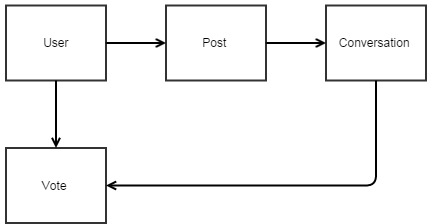
\includegraphics{diagrams/Overview-UML}}

\section{Detailed Class Diagrams}
    \subsection{Data Classes}
        \subsubsection{User Class}

            \centerline{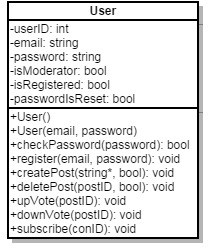
\includegraphics{diagrams/user-UML}}

            \begin{itemize}
                \item \texttt{User()} --- Default constructor. This is called to create an unregistered user.  A value for userID is assigned and stored.
                \item \texttt{User(email, password)} --- Constructor. Checks database for already existing email. If the email isn't found, creates a registerd user. Assigns values to userID, email, and password respectively. If it is already in the database, it prints an error message
                \item \texttt{isModerator()} --- Returns true if user is a moderator
                \item \texttt{isRegistered()} --- Returns true if a user is registered
                \item \texttt{checkPassword(password):bool} --- Used to login. Takes the password as plain text, hashes it and checks to see if it matches the hashed value in the database.  Returns true on success and false on failure.
                \item \texttt{register(email, password)} --- Allows an unregistered user to become a registered user on compeletion. Checks database to make sure username is available.
                \item \texttt{createPost(string*, bool):void} --- Creates a post with a reference to an image.  If the bool value is true, it creates a new conversation. If not it adds to an old conversation.
                \item \texttt{deletePost(postID, bool):void} --- Calls isModerator() to make sure user has permission to delete posts. Deletes post from database. If boolean value is true then it deletes the conversation as well.
                \item \texttt{upVote(postID)}:void --- Increments a post's score.
                \item \texttt{downVote(postID)}:void --- Decrements a post's score.
                \item \texttt{subscribe(conID)}:void --- Sends a user notification updates when they are active in a conversation.  Notification is sent when a new post is added to the conversation.
            \end{itemize}

        \subsubsection{Post Class}

            \centerline{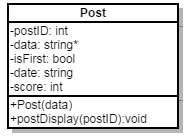
\includegraphics{diagrams/post-UML}}

            \begin{itemize}
                \item \texttt{Post(data)} --- Constructor.  Creates a Post object and assigns its data attribute to a reference of the image. It also generates a post ID and a date and stores them on creation.
                \item \texttt{postDisplay(postID):void} --- Displays the Post with the specified id.
            \end{itemize}

        \subsubsection{Conversation Class}

            \centerline{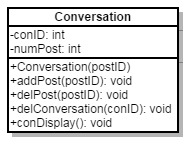
\includegraphics{diagrams/conversation-UML}}

            \begin{itemize}
                \item \texttt{Conversation(postID)} --- Constructor. Creates a new convesation with the postID passed to it.  Updates the value of numPost and assigns a value conID.
                \item \texttt{addPost(postID):void} --- Adds a new post to the conversation, a reply. Updates the value of numPost.
                \item \texttt{delPost(postID):void} --- Deletes a post from the conversation. IF the post is first, calls delConversation(). Updates the value of numPost.
                \item \texttt{delConversation(conID):void} --- Deletes all the posts from a conversation and then deletes conversation itself.
                \item \texttt{conDisplay(conID):void} --- Displays the collection of Posts in the conversation container.
            \end{itemize}

        \subsubsection{Vote Class}

            \centerline{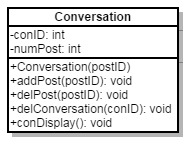
\includegraphics{diagrams/conversation-UML}}

            \begin{itemize}
                \item \texttt{Vote(user, con)} --- Constructor. Creates a vote object with attributes that reference a user ID and a conversation ID. The user will be sent a notification if someone upVotes,downVotes, or replys to a thread they are in.
            \end{itemize}

\section{Sequence Diagrams}
    \subsection{Register Sequence Diagram}
        \centerline{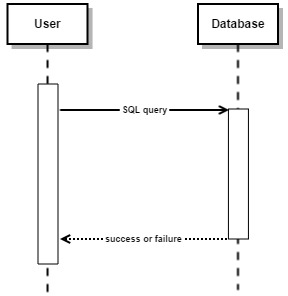
\includegraphics[width=\textwidth,height=3in,keepaspectratio]{diagrams/register-SEQ.png}}

    \subsection{Post Picture Sequence Diagram}
        \centerline{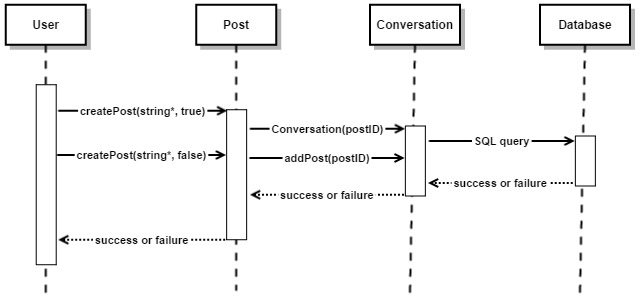
\includegraphics[width=\textwidth,height=3in,keepaspectratio]{diagrams/post-SEQ.png}}

\newpage

    \subsection{Upvote Sequence Diagram}
        \centerline{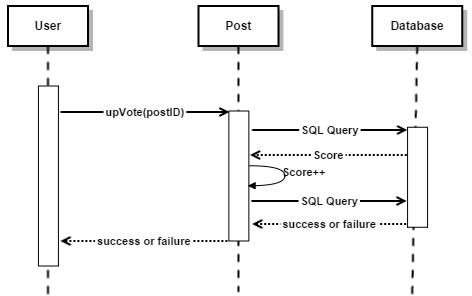
\includegraphics[width=\textwidth,height=3in,keepaspectratio]{diagrams/upvote-SEQ.png}}

    \subsection{Downvote Sequence Diagram}
        \centerline{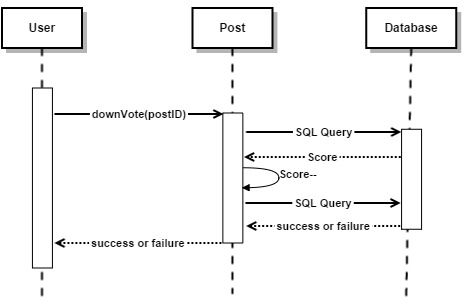
\includegraphics[width=\textwidth,height=3in,keepaspectratio]{diagrams/downvote-SEQ.png}}

\newpage

    \subsection{Remove Sequence Diagram}
        \centerline{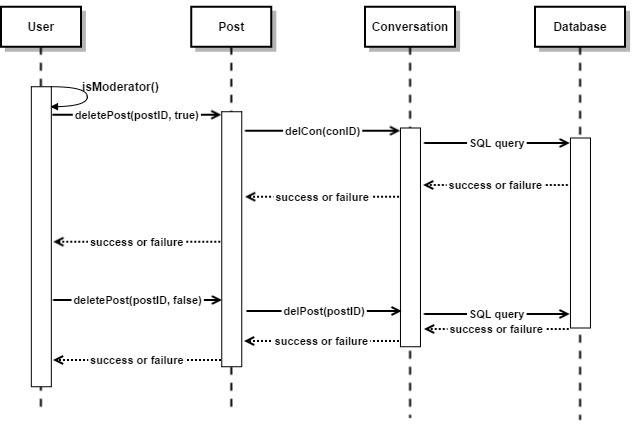
\includegraphics[width=\textwidth,height=3in,keepaspectratio]{diagrams/delete-SEQ.png}}

    \subsection{Subscribe to Updates Sequence Diagram}
        \centerline{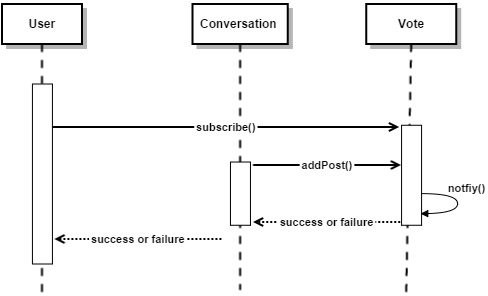
\includegraphics[width=\textwidth,height=3in,keepaspectratio]{diagrams/subscribe-SEQ.png}}

\appendix


\clearpage
\section{Task \& Role Assignments}
    \begin{description*}
        \item[Server Backend:] Kevin Stephens
        \item[Server Frontend:] Collin Kelso
        \item[Android client application:] George Hilliard
    \end{description*}

\end{document}

